Consider
\begin{equation}
g(\lambda) = \min_{C\subset V, C\neq \emptyset} \{ H(C) + \lambda\abs{C}\}
\end{equation}
where $H(C) = f(C) - \sum_{i\in C} f(\{i\})$, $f(C)$ is submodular, and $f\{i\}$ is modular.
$H(C)=0$ for $\abs{C}=1$.

The function defined in the above equation is piecewise linear about $\lambda$.

The largest turning point is equal to $\gamma_N$, which is the last critical value.

From the property of 
\begin{equation}
J_T(Z_V) = \frac{1}{\abs{V}-1} [\sum_{i \in V}()]
\end{equation}
The last line segment of $g(\lambda)$ is simply $\lambda$ itself.

\begin{figure}[!ht]
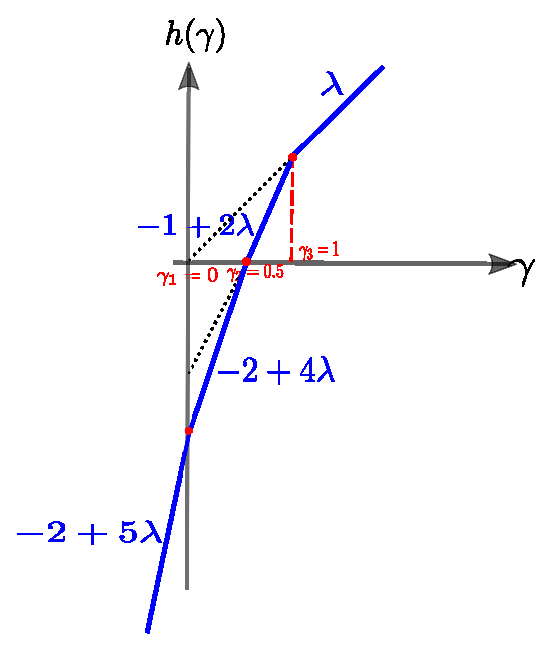
\includegraphics[width=6cm]{pic/dt2.eps}
\end{figure}
